\section{Feature-Family and Temporal Completeness Evidence}
\label{sec:mechanism_temporal}

\subsection{Interaction-Family Localization}
Family-restricted comparisons localize the positive increment to the non-focal interaction family: $M_{P+E_{\mathrm{interact}}}$ yields $\Delta\text{AP} = +0.0161$ ($95\%$ CI $[+0.0057, +0.0264]$). Adding static features alone does not improve AP ($\Delta\text{AP} = -0.0056$), while adding composition features yields a small decrease ($\Delta\text{AP} = -0.0067$). These nested comparisons are consistent with interaction summaries accounting for the observed increment within the evaluated model family; they do not identify a causal mechanism or establish that map and composition context are generally irrelevant.

\subsection{Scenario Profile Temporal Completeness}
We use scenario profiles as a temporal completeness check, not as the primary estimand. For each proxy $i$, we compute its scenario mean $\bar{E}_{s,i} = T_s^{-1} \sum_t E_{s,t,i}$. From continuous frame severity $C_{s,t}$ and TTC, we form three target profiles: $D_s^{\mathrm{Peak}} = \max_t C_{s,t}$, $D_s^{\mathrm{AUC}} = \sum_t C_{s,t}\Delta t$, and $D_s^{\mathrm{TET3}} = \sum_t \mathbb{1}[\mathrm{TTC}_{s,t} \le 3\text{ s}]\Delta t$. Separate Ridge models with $\alpha=1$, fitted on development scenario means of $P_{\mathrm{clean}}$, residualize $\bar{E}_{s,i}$ and each target profile. We report holdout Spearman correlations between the corresponding residuals with scenario-level bootstrap intervals.

\begin{figure}[t]
\centering
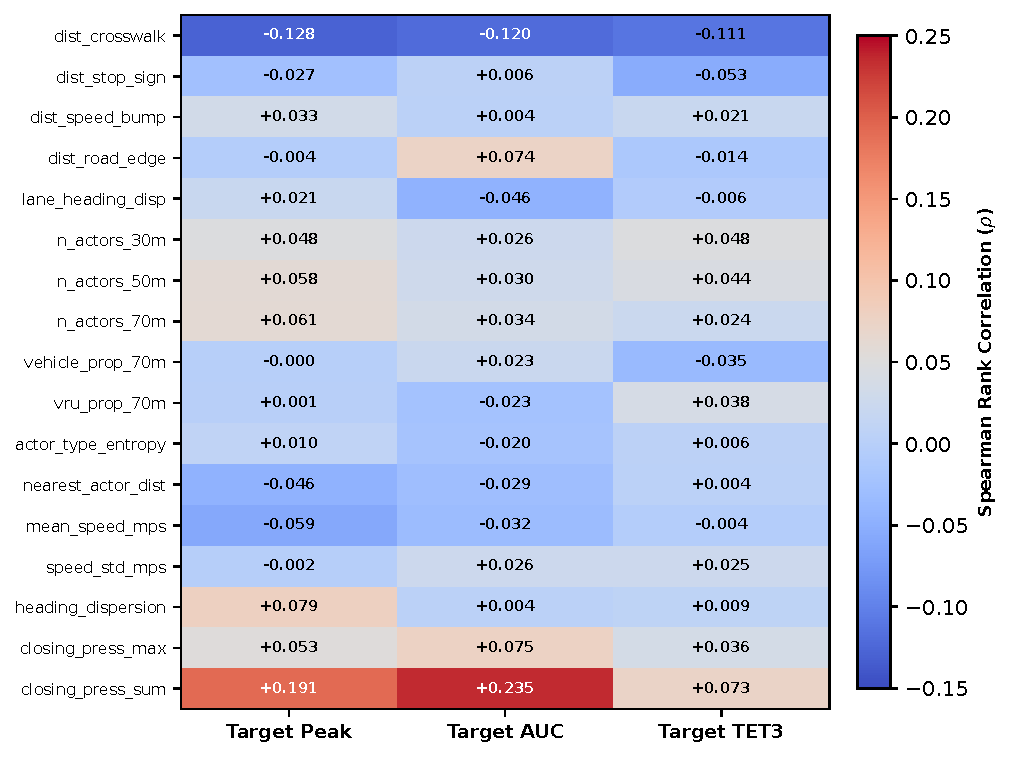
\includegraphics[width=\columnwidth]{figures/fig4_scenario_temporal_effect_heatmap.pdf}
\caption{\textbf{Temporal Target-Profile Completeness.} Holdout residual Spearman associations between each scenario-mean ODD-context proxy and target Peak, AUC, and TET3 after development-fitted adjustment for scenario-mean focal kinematics ($N=2,804$ scenarios). Column labels refer to target profiles, not transformations of the proxy itself.}
\label{fig:scenario_heatmap}
\end{figure}

The pre-specified closing-pressure-sum anchor is positive at the frame level ($\rho = +0.1712$) and for target Peak ($+0.1914$, $95\%$ CI $[+0.1549, +0.2300]$), target AUC ($+0.2345$, $[+0.2040, +0.2677]$), and target TET3 ($+0.0728$, $[+0.0405, +0.1086]$). These results support anchor-level temporal completeness, but the heterogeneous magnitudes---particularly the smaller TET3 association---and the mixed 17-feature taxonomy warrant a feature-dependent, not uniformly strong, conclusion. Across the full 17-feature taxonomy, 8 features are classified as \texttt{CROSS\_LEVEL\_STABLE}, 6 as \texttt{UNSUPPORTED\_BOTH}, 1 as \texttt{FRAME\_LOCAL}, 1 as \texttt{DISCORDANT\_SIGN}, and 1 as \texttt{TEMPORAL\_EXPOSURE\_SPECIFIC}.
